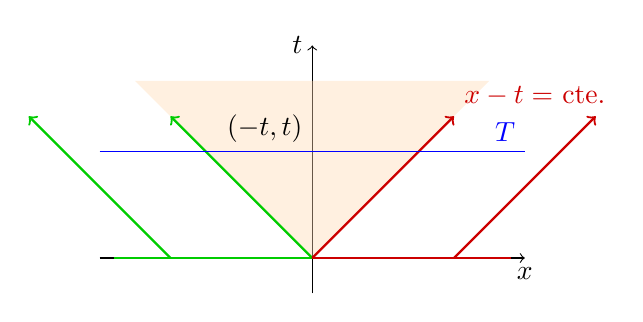
\begin{tikzpicture}[scale = 0.9]

\draw[->] (-3, 0) -- (3,0) node[below] {$x$};
\draw[->] (0, -0.5) -- (0,3) node[left] {$t$};

\draw[green!80!black, thick] (-2.8,0) -- (0,0);
\draw[red!80!black, thick] (0,0) -- (2.8,0);

\fill[orange!30!white, opacity = 0.4] (0,0) -- (-2.5,2.5) -- (2.5,2.5) -- cycle;
\draw[green!80!black, thick, ->] (0,0) -- (-2,2);
\draw[red!80!black, thick, ->] (0,0) -- (2,2) node[above right] {$x-t = $ cte.};
\draw[green!80!black, thick, ->] (-2,0) -- (-4,2);
\draw[red!80!black, thick, ->] (2,0) -- (4,2);

\draw (0,1.5) node[above left] {$(-t,t)$};
\draw[blue] (-3,1.5) -- (3,1.5) node[above left] {$T$};

\end{tikzpicture}
